\section{DNS}

\begin{defi}{DNS}
    Socket-basierte Kommunikation nutzt IP-Adressen.

    Im Gegensatz dazu wollen Endanwender sprechende Bezeichnungen, die leicht zu merken sind und Rückschlüsse auf ihre Bedeutung haben.
    Des Weiteren können sich IP-Adressen ändern, wenn z. B. ein Dienst umzieht.

    Um diese Anforderungen zu erfüllen, wurde ein System entwickelt um Namen zu übersetzen bzw. aufzulösen.

    \emph{Domain Name System (DNS)} ist eine verteilte Datenbank, welche als Serverprozess auf UDP Port 53 reagiert.
    Jeder Namensraum ist verantwortlich für sein Segment.

    Zur Geschwindigkeitsoptimierung werden angefragte Daten von Clients zwischengespeichert, wenn der DNS Server bei übergeordneten DNS Servern anfragt.

    Die IP-Adresse des DNS-Servers muss in jeden Host manuell oder via DHCP eingetragen werden.
\end{defi}

\begin{example}{DNS}
    \begin{center}
        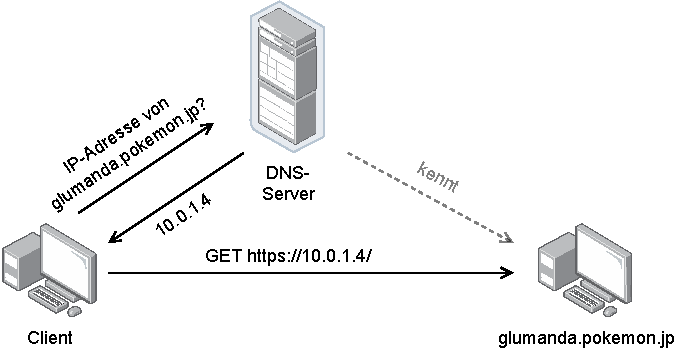
\includegraphics[width=0.75\textwidth]{includes/figures/example_dns.pdf}
    \end{center}
\end{example}

\begin{defi}{Domäne}
    Symbolische Namen bestehen aus dem Hostnamen und der Domäne.
    Die Domäne besteht aus der \emph{Top Level Domain} und potentiellen \emph{Subdomains}.

    Zur Strukturierung lassen sich die Informationen als Baum darstellen.\footnote{Die einzelnen Labels haben eine Länge von einem bis 63 Bytes.}

    Der gesamte Name (\emph{Full Qualified Domain-Name (FQDN)}) darf dabei die Länge von 255 Bytes nicht überschreiten.

    Jedes Blatt besitzt eine eindeutige IP-Adresse.
\end{defi}

\begin{example}{Domäne}
    \begin{center}
        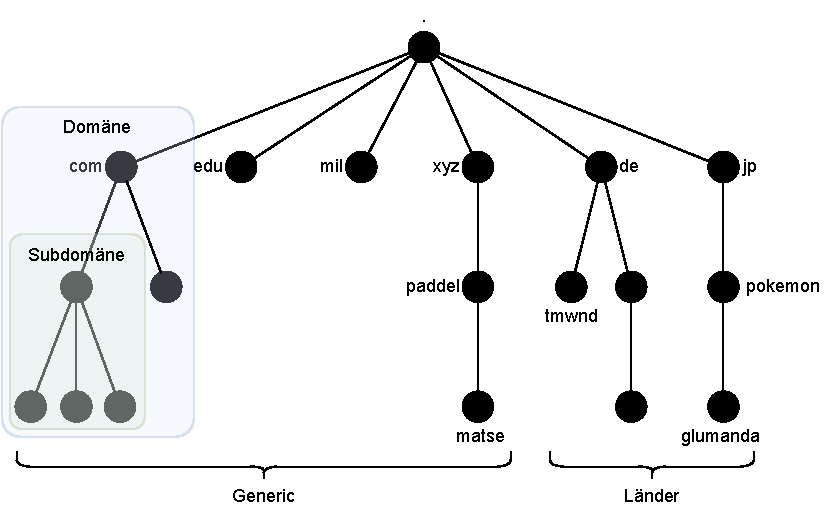
\includegraphics[width=\textwidth]{includes/figures/example_domains.pdf}
    \end{center}
\end{example}

\begin{defi}{Zone}
    Eine \emph{Zone} ist ein autarker und gemeinsam administrierter Bereich im DNS-Namensraum mit eigener Datenbank.

    Jede Zone hat einen primären und beliebig viele sekundäre Nameserver.

    \begin{itemize}
        \item Jeder Namensserver kennt nur einen Ausschnitt des gesamten Namensraums
        \item Jeder Nameserver kennt alle IP-Adressen seiner direkt untergeordneten Sub-Domains.
        \item Sekundäre Nameserver führen periodisch Updates ihrer Datenbasis durch.
        \item Der primäre Namensserver kennt den vollständigen Datenbestand.
    \end{itemize}

    Zur Einrichtung einer Zone muss man den übergeordneten Knoten davon überzeugen, die Verwaltung zu delegieren.
\end{defi}

\begin{defi}{Root-Nameserver}
    \emph{Root-Nameserver} bilden die Wurzel der hierarchischen DNS-Struktur.
    Es gibt Weltweit 13 Root-Nameserver.

    z. Zt. \texttt{\{a-m\}.root-server.net}
\end{defi}

\begin{defi}{Namensauflösung}
    Der DNS-Server beginnt bei dem Nameserver der hintersten bekannten Zone die Suche.
    Sollte er keine Daten im Cache haben, ist dies der nächste Root-Nameserver.

    Der angesprochene Nameserver kann den Client entweder zum nächsten Nameserver weiterleiten (iterativ) oder dort selber anfragen (rekursiv).
\end{defi}

\begin{example}{Namensauflösung}
    \emph{Beispiel 1:}

    Ein Client fragt bei seinem lokalen DNS die IP-Adresse des Hosts \texttt{glumanda.pokemon.jp} an.

    Da der DNS-Server keine Daten gespeichert hat, fragt er den Root-Nameserver nach der IP-Adresse.
    Dieser leitet ihn weiter auf den DNS-Server von \texttt{jp}.

    Der Nameserver von \texttt{jp} kennt den exakten Host ebenfalls nicht und leitet unseren DNS Server auf \texttt{pokemon.jp} weiter.
    Dieser kennt den Host und antwortet mit der IP-Adresse \texttt{10.0.1.4}.

    Die IP-Adresse wird von dem DNS an den Client weitergeleitet.

    \emph{Beispiel 2:}

    Nach dem ersten Beispiel fragt ein zweiter Client nach der IP-Adresse von \texttt{pikachu.pokemon.jp}.

    Da unser DNS-Server den Nameserver von \texttt{pokemon.jp} zwischengespeichert hat, fragt er direkt dort an und erhält die IP-Adresse \texttt{10.0.1.22}.

    Diese wird erneut an den Client weitergeleitet.
\end{example}

\begin{bonus}{Weitere DNS-Dienste}
    Neben der Auflösung von Namen ist der DNS-Server zuständig für:
    \begin{itemize}
        \item Die Weiterleitung zu dem Mail-Server der Zone (\emph{Mail Exchange Resource Record} (MX-RR))
        \item Die Weiterleitung zu IP-Telefon Kommunikationspartnern
        \item Caching von Anfragen
    \end{itemize}
\end{bonus}

\begin{bonus}{DNS-Datenbank}
    In der \emph{DNS-Datenbank} befinden sich folgende Typen von Einträgen:

    \begin{tabular}{|l|l|l|}
        \hline
        Typ   & Bedeutung                & Wert                                    \\\hline\hline
        SOA   & Start of Authority       & Parameter für diese Zone                \\\hline
        A     & IPv4-Adresse eines Hosts & 32 bit Integer                          \\\hline
        AAAA  & IPv6-Adresse eines Hosts & 128 bit Integer                         \\\hline
        MX    & Mail-Exchange            & Priority, domain willing to accept Mail \\\hline
        NS    & Name-Server              & Name des Name-Servers des Namensraums   \\\hline
        CNAME & Canonical Name           & (Sub-) Domain Name                      \\\hline
        PTR   & Pointer                  & Alias für eine IP-Adresse               \\\hline
        SPF   & Sender policy framework  & Text encoding für Mails Policy          \\\hline
        SRV   & Service                  & Host, auf dem der Service läuft         \\\hline
        TXT   & Text                     & Kommentare                              \\\hline
    \end{tabular}
\end{bonus}

\begin{example}{DNS-Datenbank}
    Die imaginäre Datenbank des Nameservers von \texttt{pokemon.jp}

    \begin{center}
        \begin{tabular}{TTTTT}
            pokemon.jp   & 86400 & IN & NS    & pokemon-dns \\
            feuerpokemon & 86400 & IN & CNAME & pokemon.jp  \\
            \\
            eich         & 86400 & IN & A     & 10.0.255.1  \\
            esche        & 86400 & IN & A     & 10.0.255.2  \\
            \\
            pokemon      & 86400 & IN & MX    & 1 eich      \\
            pokemon      & 86400 & IN & MX    & 2 esche     \\
            \\
            glumanda     & 86400 & IN & A     & 10.0.1.4    \\
            glumanda     & 86400 & IN & AAAA  & ::4         \\
            pikachu      & 86400 & IN & A     & 10.0.1.22   \\
        \end{tabular}
    \end{center}
\end{example}

\begin{bonus}{DNS-Attacken}
    DNS ist ein zentraler Bestandteil eines Netzwerks und ein kritischer Dienst.

    Da er nur UDP verwendet, ist er häufig Angriffsziel.

    \begin{itemize}
        \item \emph{DNS Spoofing}:
              Durch Manipulation (Maskierung) werden Benutzer für Phishing-Attacken auf falsche Webseiten gelenkt.
        \item \emph{Cache Poisoning}:
              Der Cache des DNS Servers wird vergiftet, in der Hoffnung, dass Clients den Cache unhinterfragt in ihren Cache übernehmen.
        \item \emph{DDoS}
    \end{itemize}

    Um diese Angriffe zu verhindern gibt es verschiedene Sicherheitserweiterungen\footnote{z. B. \emph{DNS over TLS}}.
\end{bonus}

\begin{bonus}{DNS-Filter}
    DNS-Anfragen können mit einem Proxy gefiltert werden, um z. B. unerwünschte Anfragen abzubrechen (z. B. auf Werbeseiten).

    Beispielsweise lässt sich ein Raspberry Pi mittels \emph{Pi-Hole} zu solch einem DNS-Proxy umfunktionieren.

    Erwünschte Anfragen könnte man z. B. auf den Google-DNS-Server \texttt{8.8.8.8} weiterleiten, oder seinen lokalen Nameserver des Routers nutzen.
\end{bonus}